\documentclass[10pt]{article}
\usepackage[utf8]{inputenc}
\usepackage{amsmath}
\usepackage{authblk}
\usepackage{amssymb}
%\usepackage{lucidbry}
\usepackage{graphicx}
\usepackage{latexsym}
\usepackage{subcaption}
\usepackage{physics}
\usepackage[dvipsnames]{xcolor}
\usepackage{tikz,tikzsettings}
\usepackage{verbatim}
\usetikzlibrary{arrows,shapes}
\usepackage{amssymb}
\usepackage{amsmath}
\usepackage{verbatim}
\usepackage{float}
\usepackage{units}
\usepackage[round]{natbib}
\usepackage[english]{babel}
\bibliographystyle{plainnat}
%\setcitestyle{numeric,open={(},close={)}} \usepackage{color}
%\usepackage{colortbl}
\usetikzlibrary{decorations.markings}
\usetikzlibrary{decorations.pathreplacing}
\usetikzlibrary{shapes,calc,backgrounds,arrows,fit,decorations.pathmorphing,matrix}
\usepackage[margin=0.79in]{geometry}

\graphicspath{{./}{./figures/}{./figures/paper/}}

\newcommand{\Is}{\bm{\mathrm{I}}} % Resources.
\newcommand{\Js}{\bm{\mathrm{J}}} % Units.
\newcommand{\Ks}{\bm{\mathrm{K}}} % Resources.
\newcommand{\Ms}{\bm{\mathrm{M}}} % Transition catalog.
\newcommand{\Ns}{\bm{\mathrm{N}}} % Transition counter.

\newcommand{\useq}{\mathbf{u}} \newcommand{\xseq}{\mathbf{x}}
\newcommand{\bbR}{\mathbb{R}} \newcommand{\bbW}{\mathbb{W}}
\newcommand{\bbU}{\mathbb{U}} \newcommand{\bbI}{\mathbb{I}}
\newcommand{\bbX}{\mathbb{X}} \newcommand{\bbP}{\mathbb{P}}

\title{Nonlinear system identification using machine learning tools}
\author{Pratyush Kumar}
\date{\today}

\begin{document}

\maketitle

\section{Process modeling}
We consider the problem of system identification of the following nonlinear
plant:
\begin{align*}
  x_p^+ &= f_p(x_p, u, w) \\
  y &= h_p(x_p) + v
\end{align*}
in which $x_p \in \bbR^{n_p}$ is the plant state, $u \in \bbU \subset \bbR^m$ is
the manipulated control input, $y \in \bbR^p$ is the measurement, $w$ is the
process noise, and $v$ is the measurement noise. The objective of developing the
model is to use it subsequently in model predictive control (MPC). Therefore, we
consider several types of grey-box, hybrid, and black-box models and analyze
their predictive capabilities as well as their usefulness for online
optimization in MPC. 

\section{Model architectures for system identification}
We describe several process modeling frameworks which determine parameters in
their proposed model architecture by minimizing the multi-step ahead prediction
error of the model on training data. A nonlinear optimization problem is solved
for this identification step. The estimated parameters define the model, which
is then used subsequently to perform model validation and for use in MPC.

\subsection{Grey-box model}
We first consider the grey-box modeling strategy, which is the current
industrial state-of-the-art system identification technique. A parameterized
model is defined based on first-principle knowledge about the plant, and
parameters in the model are estimated from training data by solving the
prediction-error minimization problem. The grey-box model is typically defined
in continuous time and is of the following form:

\begin{align*}
  \dot{x}_g &= f_g(x_g, u, \theta_g) \\
  y &= h_g(x_g, \theta_g)
\end{align*}

The following nonlinear program (NLP) is solved to identify the parameters
$\theta_g$:

\begin{align} \label{eq:gb_training}
  \underset{x_g^i(0), \ \theta_g}{\textnormal{min}} \sum_{i=1}^{N_{tr}} \sum_{k=1}^{N_t} 
  \dfrac{1}{N_tN_{tr}} &\norm{\tilde{y}^i(k) - y^i(k)}^2_{R_v^{-1}}  \\
  \textnormal{subject to} \quad \quad x_g^{i+} &= f_{gd}(x_g^i, u^i, \theta_g) \nonumber \\
   \tilde{y}^i &= h_g(x_g^i, \theta_g) \nonumber
\end{align}

in which $\theta_g$ and $x_g^i(0)$ are the decision variables in the
optimization problem, which are parameters in the grey-box model and initial
state used for forecasting the predicted measurements respectively. We assume
that multiple trajectories can be used in the training data, and the superscript
$i$ is used to denote the trajectory number. We use $N_{tr}$ to denote the total
number of trajectories in training data and $N_t$ to denote the number of
samples in each trajectory. The function $f_{g}(\cdot)$ is discretized at the
measurement sample time to obtain the function $f_{gd}(\cdot)$ that is used to
make forecasts in the above optimization.

\subsection{Hybrid model}

Often in industrial applicationns, first-principle knowledge about the plant is
incomplete. Hence, grey-box system identification and subsequent use of the
grey-box model in real-time optimization can lead to suboptimal economic
performance. We propose to augment the grey-box model using a neural network
(NN) such that the overall hybrid model can capture any unknown process dynamics
in the plant, therefore leading to improved economic performance when used
subsequently in real-time optimization. We define this hybrid model as follows:

\begin{align*}
  x_g^+ &= f_{gd}(x_g, u, \theta_g) + f_N(z, u, \theta_N) \\
  z^+ &= f_z(x_g, z, u) \\
  y &= h_g(x_g, \theta_g)
\end{align*}
in which $f_N(\cdot)$ is a NN and $\theta_N$ denotes the parameters in the
network. We use $z$ to denote the vector of past measurements and control
inputs. This vector is considered as an additional state in the overall dynamic
model and is defined as follows:
\begin{align} \label{eq:pastyu}
  \mathbf{y}_{k-N_p:k-1} &= [y(k-N_p)', ... \ , y(k-1)']' \nonumber \\
  \mathbf{u}_{k-N_p:k-1} &= [u(k-N_p)', ... \ , u(k-1)']' \nonumber \\
  z(k) &= [\mathbf{y}_{k-N_p:k-1}', \mathbf{u}_{k-N_p:k-1}']'
\end{align}
in which $N_p$ is the number of past measurements and control inputs used. The
function $f_z(\cdot)$ describes the dynamics of the state $z$ and its structure
is defined as follows: 
\begin{align*}
  f_z(x_g, z, u) = \begin{bmatrix}
    y(k-N_p+1) \\
    y(k-N_p+2) \\
    \vdots \\
    h_g(x_g, \theta_g) \\
    u(k-N_p+1) \\ 
    u(k-N_p+2) \\
    \vdots \\
    u(k)
  \end{bmatrix}
\end{align*}
We assume that the parameters in the grey-box model are first estimated by
solving the NLP \eqref{eq:gb_training}, and the following similar NLP is solved
to determine parameters ($\theta_N$) in the NN.

\begin{align} \label{eq:hybrid_training}
  \underset{\theta_N}{\textnormal{min}} \sum_{i=1}^{N_{tr}} \sum_{k=1}^{N_t} 
  \dfrac{1}{N_tN_{tr}} &\norm{\tilde{y}^i(k) - y^i(k)}^2  \\
  \textnormal{subject to} \quad \quad x_g^{i+} &= f_{gd}(x_g^i, u^i, \theta_g) + f_z(z^i, u^i, \theta_N) \nonumber \\
  z^{i+} &= f_z(x_g^i, z^i, u^i) \nonumber \\
   \tilde{y}^i &= h_g(x_g^i, \theta_g) \nonumber
\end{align}
The stochastic gradient descent algorithm Adam is used to solve the above
optimization using the software tensorflow. Note that we do not estimate the
initial grey-box state for each trajectory in the optimization problem, and fix
those states heuristically to make forecasts during the optimization process.
The control inputs and measurements are scaled as $u := (u -
u_{\textnormal{MEAN}})/u_{\textnormal{STD}}$ and $y := (y -
y_{\textnormal{MEAN}})/y_{\textnormal{STD}}$, in which $u_{\textnormal{MEAN}}$
and $y_{\textnormal{MEAN}}$ are the respective means computed on training data.
Similarly, $u_{\textnormal{STD}}$ and $y_{\textnormal{STD}}$ are the respective
standard deviations. Due to this scaling, we do not consider the penalty
$R_v^{-1}$ in the training objective.

\subsection{Black-box models}
Next, we consider black-box system identification strategies which do not impose
any a-prior knowledge about the plant and develop the dynamic model purely from
data. We consider two types of black-box models in this section: NNs and dynamic
models based on the Koopman operator theory. The latter type of model is
considered based on the motivation that it imposes a linear structure on the
dynamics in a high-dimensional space, therefore leading to a linear or quadratic
program to be solved online in MPC.

\subsubsection{Neural network}
The black-box NN uses the vector of past measurements and control inputs $z$
\eqref{eq:pastyu} as the state in the dynamic model and is structured as follows
\begin{align} \label{eq:bbnn_model}
  z^+ &= f_z(z, u) \\ 
  y &= h_N(z, \theta_N) \nonumber
\end{align}
in which $h_N(\cdot)$ is a NN and $\theta_N$ are the parameters in the network.
The function $f_z(\cdot)$ denotes the dynamics of the state $z$ and is defined
as 

\begin{align*}
  f_z(z, u) = \begin{bmatrix}
    y(k-N_p+1) \\
    y(k-N_p+2) \\
    \vdots \\
    h_N(z, \theta_N) \\
    u(k-N_p+1) \\ 
    u(k-N_p+2) \\
    \vdots \\
    u(k)
  \end{bmatrix}
\end{align*}

\subsubsection{Koopman operator model}

The Koopman model represents the dynamics as a linear system in a
high-dimensional state-space that is a nonlinear transformation of the original
state-space. This transformation is chosen such that the input-output behavior
is linear. The overall dynamic model is represented as:

\begin{align} \label{eq:koop_model}
  x_{kp} &= [y', z', f_N(y, z, \theta_N)']' \\
  x_{kp}^+ &= Ax_{kp} + Bu \nonumber \\
  y &= [I, \ 0] x_{kp} \nonumber
\end{align}
in which $x_{kp} \in \bbR^N$ is the state in a high-dimensional state-space,
$f_N(\cdot)$ is a NN used for the nonlinear transformation, and $\theta_N$
denotes the parameters in the network.

\subsubsection{Training}
The training optimization problem for both the black-box NN and the Koopman
operator model is to minimize the mean-squared-error (MSE) similar to the
nonlinear program \eqref{eq:hybrid_training}. The model equality constraints are
replaced with the equations \eqref{eq:bbnn_model} and \eqref{eq:koop_model} for
the black-box and Koopman operator model respectively. The measurements and
control inputs are scaled using the mean and standard deviation computed from
the training data. The initial state to make model predictions in the
optimization process is set based on a window of past measurements and control
inputs in the training data.

\section{Two reaction system example}

We now study the performance of the modeling frameworks on a simple two
reaction system example in three steps. First, we examine the predictive
capability of the developed models on open-loop validation data. Second, we
analyze the steady-state optimum with an economic stage cost. Finally, we
analyze the optimal control input profiles on a dynamic economic optimization
problem. These three steps shed light on the predictive abilities of the models
and their usefulness for real-time optimization in the operation of chemical
processes.

The following plant model with two reactions $A \rightarrow B$ and $3B
\rightleftharpoons C$ is considered:
\begin{align*}
  \dfrac{dC_A}{dt} &= \dfrac{C_{Af} - C_A}{\tau} - k_1C_A\\
  \dfrac{dC_B}{dt} &= k_1C_A - 3k_2C^3_B + 3k_3C_C- \dfrac{C_B}{\tau}\\
  \dfrac{dC_C}{dt} &= k_2C^3_B - k_3C_C - \dfrac{C_C}{\tau}
\end{align*}

in which, $C_A$, $C_B$, and $C_C$ are the concentrations of the three species
$A$, $B$, and $C$. The parameters $k_1$, $k_2$, and $k_3$ are the rate constants
and the $\tau$ is the residence time.

The grey-box model is built as follows based on an assumption that the knowledge
of the second side reaction ($3B \rightleftharpoons C $) is not available:
\begin{align*}
  \dfrac{dC_A}{dt} &= \dfrac{C_{Af} - C_A}{\tau} - k_1C_A\\
  \dfrac{dC_B}{dt} &= k_1C_A - \dfrac{C_B}{\tau}
\end{align*}

The rate constants and residence time in both the models are set to $k_1 = 1 \
\textnormal{m}^3/\textnormal{min}$, $k_2 = 0.01 \
\textnormal{m}^3/\textnormal{min}$, $k_3 = 0.05 \
\textnormal{m}^3/\textnormal{min}$, and $\tau = 5 \ \textnormal{min}$. The
sample time for the measurements is $1 \ \textnormal{min}$, and we assume that
only the concentrations of the species $A$ and $B$ are measured in real-time.

\subsection{Model validation}
In the simulations for this example, we fix the grey-box model parameters
heuristically and only train the two black-box models: NN and Koopman operator
model. We generate 1 day (1440 samples) of data by simulating the plant model
with a Pseudo-random-binary-signal (PRBS) control input profile. The generated
data is split into 12 hours of training data, 6 hours of buffer data, and 6
hours of validation data. The MSE metric is monitored on the buffer data during
the training process, and model weights are updated only when MSE decreases on
the buffer dataset. After the training step, the black-box NN and Koopman
operator models are used to make predictions on the validation data shown in
Figure \ref{fig:tworeac_validation}. We observe good quality measurement
predictions with both types of dynamic black-box models.

\begin{figure}[!h]
  \centering
  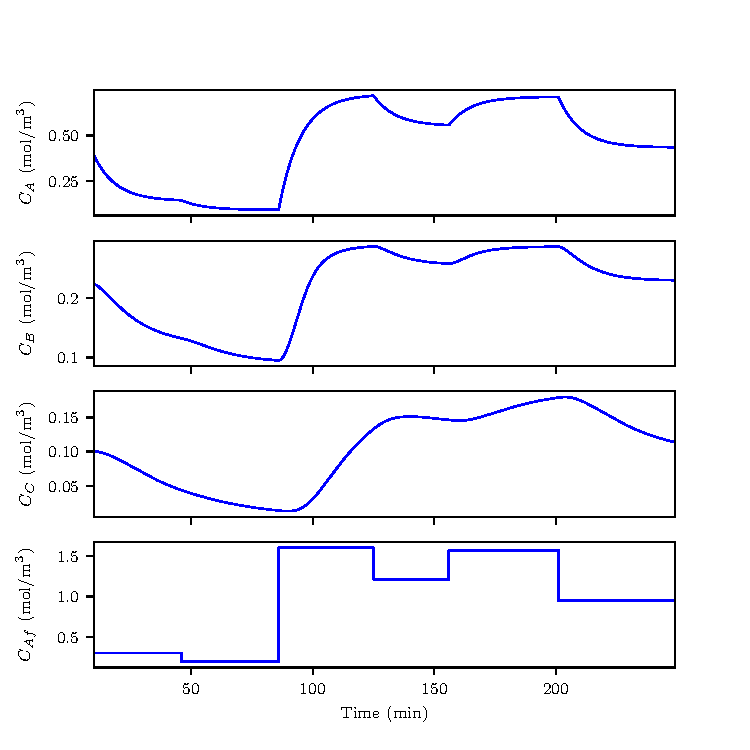
\includegraphics[page=1, height=0.5\textheight,
                   width=0.7\textwidth]{tworeac_plots.pdf}
  \caption{Model validation on open-loop data with the black-box NN and Koopman operator model.}
  \label{fig:tworeac_validation}
\end{figure}

\subsection{Steady state optimization}
The two trained black-box NN and Koopman operator model are used in a
steady-state optimization problem to determine the economically optimal steady
state of the system. In a typical chemical plant, this type of optimization is
solved periodically every few hours based on changes in raw material costs and
product selling prices. The obtained steady state is sent to lower-level control
layers such as model predictive control (MPC) or the
proportional-integral-derivative (PID) controller. The optimization problem
solved is:
\begin{align} \label{eq:ss_opt}
  \underset{u_s}{\textnormal{min}} & \quad \ell(y_s, u_s) \\
  x_s &= f(x_s, u_s) \nonumber \\ 
  y_s &= h(x_s) \nonumber \\
  \underline{u} \leq &u_s \leq \overline{u} \nonumber
\end{align}
in which the steady-state control input ($u_s$) is the decision variable,  and
the model is required to satisfy steady-state constraints. The stage cost for
the two reaction system is chosen as:
\begin{equation*}
  \ell(y_s, u_s) = p_1C_{Afs} - p_2C_{Bs}
\end{equation*}
in which $p_1$ and $p_2$ are the parameters chosen to represent the raw material
(species $A$) cost and the product (species $B$) selling price respectively. 

First, we plot the economic objective ($\ell(y_s, u_s)$) as a function of the
steady-state control input to examine the cost structure obtained with the
different models. This plot is shown in Figure \ref{fig:tworeac_sscost}.

\begin{figure}[!h]
  \centering
  \includegraphics[page=1, height=0.4\textheight,
                   width=0.6\textwidth]{tworeac_ssopt.pdf}
  \caption{Steady-state cost curve $\ell(y_s, u_s)$ as a function of the control input for the plant, grey-box, black-box NN, and Koopman operator models.}
  \label{fig:tworeac_sscost}
\end{figure}

We observe that the black-box NN model correctly captures the true plant cost
curve after training, and the grey-box and Koopman operator models do not. This
behavior by the latter two models is due to the linear structure in the dynamic
models. Upon solving the optimization problem \eqref{eq:ss_opt}, the optimum
steady-state control input ($C_{Afs}^0$) values are $1.63$, $2.5$, $1.60$, and
$2.5$ in mol/m$^3$ for the plant, grey-box, black-box NN, and Koopman operator
models respectively. The use of grey-box and Koopman operator models
subsequently in real-time optimization of chemical processes can therefore
result in suboptimal economic performance.

\subsection{Dynamic economic optimization}
The performance of the models is now studied with a dynamic economic
optimization problem. In contrast to the steady-state optimization problem
\eqref{eq:ss_opt}, operational strategies based on solving a dynamic
optimization problem aim to maximize plant profit during the transients as well
as opposed to just steady states. The economic optimization problem is:

\begin{align} \label{eq:dyn_opt}
  \underset{\useq}{\textnormal{min}} & \quad \sum_{k=0}^{N-1} \ell(y(i), u(i)) \\
  x^+ &= f(x, u) \nonumber \\ 
  y &= h(x) \nonumber \\
  x(0) &= x_0 \nonumber \\ 
  \underline{u} \leq &u \leq \overline{u} \nonumber
\end{align}

The above optimization problem is similar to the optimization solved in MPC, and
the difference is the choice of the economic stage cost $\ell(\cdot)$, which is
a setpoint tracking stage cost in a traditional MPC controller. This
optimization problem can also be solved directly at the regulatory control
layers and is often referred to as the economic MPC controller.

\begin{figure}[!h]
  \centering
  \includegraphics[page=1, height=0.5\textheight,
                   width=0.7\textwidth]{tworeac_openloop.pdf} \caption{Optimal
                   open-loop control input and state profiles after solving the
                   dynamic economic MPC problem \eqref{eq:dyn_opt} with the
                   plant, grey-box, black-box NN, and Koopman operator models.}
  \label{fig:tworeac_openloop}
\end{figure}

Before analyzing a full closed-loop simulation with the economic MPC controllers
based on the different dynamic models, we first examine the open-loop solutions
of the optimization problem \eqref{eq:dyn_opt} given one initial state. Figure
\ref{fig:tworeac_openloop} shows the open-loop state and control input profiles
for the plant, grey-box, black-box NN, and Koopman operator models. We notice
that the black-box NN has an optimal control input profile qualitatively similar
to that of the plant. Whereas, the optimal profiles for the grey-box and Koopman
operator model are different than the plant model. This simple analysis shows
that the use of the grey-box and Koopman operator models in MPC can result in
suboptimal economic performance.

%\section{Large, CSTR and flash system example}
%We next study the performance of the black-box NN modeling framework on a 
%large chemical process that consists of a chemical reactor and flash separator 
%in series. The process is depicted in Figure \ref{fig:cstr_flash}, and the 
%ordinary differential equations (ODEs) with parameter values describing the 
%plant model are shown in Appendix \ref{app:cstr_flash}. The model consists of 
%12 states ($H_r$, $C_{Ar}$, $C_{Br}$, $C_{Cr}$, $T_r$, $H_b$, $C_{Ab}$, 
%$C_{Bb}$, $C_{Cb}$, $T_b$), 6 measurements ($H_r$, $C_{Br}$, $T_r$, $H_b$, 
%$C_{Bb}$, $T_b$), and 2 control inputs ($F$, $D$). The sample time for the 
%measurements is 1 min.


%\begin{figure}[!h]
%  \centering
%  \includegraphics[page=1, height=0.5\textheight,
%                   width=0.7\textwidth]{cstr_flash.pdf}
%  \caption{Schematic of the CSTR and flash chemical process.}
%  \label{fig:cstr_flash}
%\end{figure}

%\subsection{Model validation}

% \begin{figure}[!h]
%   \centering
%   \includegraphics[page=1, height=0.5\textheight,
%                    width=0.7\textwidth]{cstr_flash_plots.pdf}
%   \caption{Schematic of the CSTR and flash chemical process.}
%   \label{fig:cstr_flash_uvalidation}
% \end{figure}

% \begin{figure}[!h]
%   \centering
%   \includegraphics[page=2, height=0.5\textheight,
%                    width=0.7\textwidth]{cstr_flash_plots.pdf}
%   \caption{Schematic of the CSTR and flash chemical process.}
%   \label{fig:cstr_flash_yvalidation}
% \end{figure}

%\subsection{Steady state optimization}

%\subsection{Dynamic economic optimization}


\section{Hybrid model}

\begin{equation*}
\begin{bmatrix}
\dfrac{dC_A}{dt} \\
\dfrac{dC_B}{dt} \\
\dfrac{dC_C}{dt}
\end{bmatrix} = \begin{bmatrix}
\dfrac{C_{Af} - C_A}{\tau} \\
- \dfrac{C_B}{\tau} \\
- \dfrac{C_C}{\tau}
\end{bmatrix} + f_N(C_A, C_B, C_C)
\end{equation*}

\section{Learn cost functions with input convex NNs}
Different proposal. NNs can be made convex from their inputs to outputs. 
Consider the following architecture (Amos, Xu, Kolter 2017) - 

\begin{equation*}
	z_{i+1} = g_i(W_i^{z}z_{i} + W_i^{y}x + b_i), i=0, 1, ...k-1
\end{equation*}

If $g_i(\cdot)$ is convex and non-decreasing, $W_0^{z} = 0$, and $W_{1:k-1}^{z}$
are all non-negative, then the NN architecture is convex, i.e, the function 
$z_k(x)$ is convex.

\textbf{RTO algorithm}
\begin{itemize}
	\item Obtain steady-state data ($u_s$, $y_s$), and samples of the cost 
	curve ($\ell(u_s, y_s, p)$) based on current economic cost parameters.
	\item Fit the input convex NN to the cost curve and optimize.
\end{itemize}

Extensions - Can allow the NN to be non-convex in some inputs and convex in 
some inputs. So the NN cost function can be non-convex in economic 
parameters/disturbance estimates, but we will force it to be convex in $u_s$.

\section*{Appendix} 
\renewcommand{\thesubsection}{\Alph{subsection}}

\subsection{CSTR and flash system model} \label{app:cstr_flash}

\begin{align*}
  \dfrac{dH_r}{dt} &= \dfrac{F + D -F_r}{A_r}\\
  \dfrac{dC_{Ar}}{dt} &= \dfrac{F(C_{Af} -C_{Ar}) +
                         D(C_{Ad} -C_{Ar})}{A_rH_r} - r_1 \\
  \dfrac{dC_{Br}}{dt} &= \dfrac{-FC_{Br} + 
                          D(C_{Bd} -C_{Br})}{A_rH_r} + r_1 -3r_2\\
  \dfrac{dC_{Cr}}{dt} &= \dfrac{-FC_{Cr} + 
  D(C_{Cd} -C_{Cr})}{A_rH_r} + r_2\\
  \dfrac{dT_r}{dt} &= \dfrac{F(T_f - T_r) + D(T_d -T_r)}{A_rH_r} + 
                      \dfrac{r_1\Delta H_1 + r_2\Delta H_2}{\rho C_p} - 
                      \dfrac{Q_r}{\rho A_r C_p H_r}\\
  \dfrac{dH_b}{dt} &= \dfrac{F_r - F_b - D}{A_b} \\
  \dfrac{dC_{Ab}}{dt} &= \dfrac{F_r(C_{Ar} -C_{Ab}) + 
                          D(C_{Ab} -C_{Ad})}{A_bH_b} \\
  \dfrac{dC_{Bb}}{dt} &= \dfrac{F_r(C_{Br} -C_{Bb}) + 
                          D(C_{Bb} -C_{Bd})}{A_bH_b} \\
  \dfrac{dC_{Cb}}{dt} &= \dfrac{F_r(C_{Cr} -C_{Cb}) + 
                          D(C_{Cb} -C_{Cd})}{A_bH_b} \\
  \dfrac{dT_b}{dt} &= \dfrac{F_r(T_r - T_b)}{A_bH_b} +
                      \dfrac{Q_b}{\rho A_b C_p H_b}\\
\end{align*}

Here, the rate of reactions $r_1$ and $r_2$ are defined as:
\begin{align*}
  r_1 = k_1^*e^{-E_1/RT_r}C_{Ar}, \quad r_2 = k_2^*e^{-E_2/RT_r}C_{Br}^3
\end{align*}

The outlet flowrates from the CSTR and flash are computed from the height of the reaction mixture in each unit as follows:
\begin{align*}
  F_r = k_r\sqrt{H_r}, \quad F_b = k_b\sqrt{H_b}
\end{align*}

The concentrations of the species in the recycle stream are computed using the following equations:
\begin{align*}
  C_{Ad} = \dfrac{\alpha_A C_{Ab}}{\sum_{i \in \{ A, B, C\}} \alpha_iC_{ib}} , \quad, C_{Bd} = \dfrac{\alpha_B C_{Bb}}{\sum_{i \in \{ A, B, C\}} \alpha_iC_{ib}}, \quad C_{Cd} = \dfrac{\alpha_C C_{Cb}}{\sum_{i \in \{ A, B, C\}} \alpha_iC_{ib}}
\end{align*}

The parameters used to simulate the model and the control input constraints used for the optimization problems are summarized in Table \ref{table:cstr_flash_pars}.

\newpage

\begin{table}[!h]
  \centering
  \begin{tabular}{|c|c|c|c|c|c|}
      \hline
      \multicolumn{6}{ |c| }{Parameters used to simulate the ODEs} \\
      \hline
      Parameter & Value & Unit & Parameter & Value & Unit\\
      \hline
      $\alpha_A$ & 8 &  & $k_1^*$ & 0.3 & \unit{min$^{-1}$}\\ 
      $\alpha_B$ & 1 &  & $k_2^*$ & 0.5 & \unit{min$^{-1}$} \\ 
      $\alpha_C$ & 1 &  & $\Delta H_1$ & 100 & \unitfrac{kJ}{mol} \\ 
      $\rho$ & 6 & \unitfrac{kg}{m$^3$} & $\Delta H_2$ & 120 &
      \unitfrac{kJ}{mol} \\ 
      $C_p$ & 3 & \unitfrac{kJ}{kg-K} & $E_1/R$ & 200 & \unit{K} \\ 
      $A_r$ & 3 & \unit{m$^2$} & $E_2/R$ & 300 & \unit{K} \\ 
      $A_b$ & 3 & \unit{m$^2$} & $T_d$ & 310 &
      \unit{K} \\ 
      $k_r$ & 4 & \unitfrac{m$^{5/2}$}{min} & $C_{Af}$ & 6 & \unitfrac{mol}{m$^3$} \\ 
      $k_b$ & 2 & \unitfrac{m$^{5/2}$}{min} &  $Q_r$ &  200 & \unitfrac{kJ}{min} \\ 
      $T_f$ & 320 & \unit{K} &  & &  \\ 
      $Q_b$ & 200 & \unitfrac{kJ}{min} & & & \\ 
      \hline       
      \multicolumn{6}{ |c| }{Actuator constraints ($\underline{u},
      \overline{u}$)} \\
      \hline
      $F$ & (5, 15) & \unitfrac{m$^3$}{min} & $D$ & (2, 8) &
      \unitfrac{m$^3$}{min}  \\ 
      \hline
  \end{tabular} \caption{Parameters used in the ODEs to simulate the plant in
  the CSTR in series with a flash separator example, and the actuator constraints
  for the optimization problems.}
\label{table:cstr_flash_pars}
\end{table}

\end{document}
